% This file was created with tikzplotlib v0.10.1.
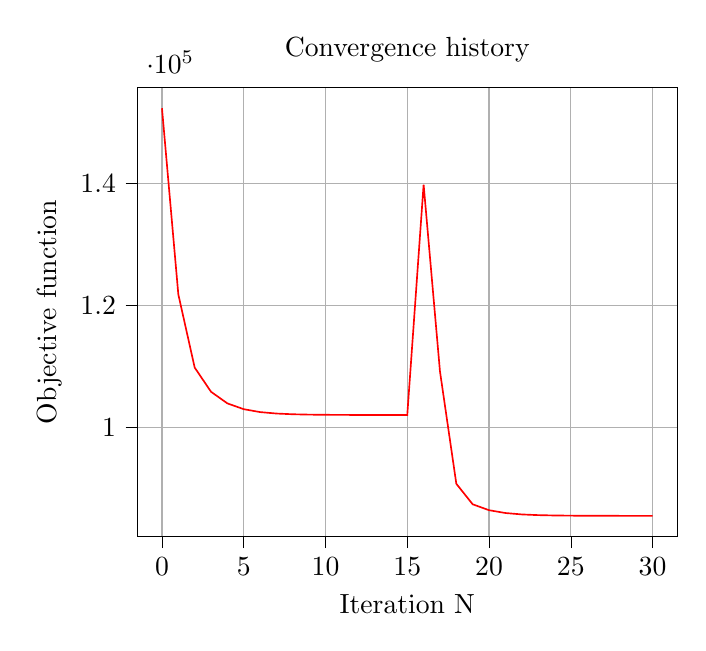
\begin{tikzpicture}

\definecolor{darkgray176}{RGB}{176,176,176}

\begin{axis}[
tick align=outside,
tick pos=left,
title={Convergence history},
x grid style={darkgray176},
xlabel={Iteration N},
xmajorgrids,
xmin=-1.5, xmax=31.5,
xtick style={color=black},
y grid style={darkgray176},
ylabel={Objective function},
ymajorgrids,
ymin=82194.8464797051, ymax=155664.759349268,
ytick style={color=black}
]
\addplot [semithick, red]
table {%
0 152325.217855197
1 121817.873085576
2 109832.479950859
3 105863.177202022
4 103961.217252771
5 103010.491043297
6 102535.12778532
7 102297.445903963
8 102178.605517514
9 102119.185536702
10 102089.475632327
11 102074.530115808
12 102067.142749969
13 102059.76660216
14 102059.765835007
15 102059.765835007
16 139814.735347427
17 109205.284321175
18 90788.8373646622
19 87425.2405707197
20 86458.0221604854
21 85996.1763349321
22 85765.281904733
23 85649.8347528423
24 85592.111124315
25 85563.2495536147
26 85548.8186808454
27 85541.6032697659
28 85534.3888985389
29 85534.3879737762
30 85534.3879737762
};
\end{axis}

\end{tikzpicture}
